\documentclass[a4paper,12pt]{book}
\usepackage{graphicx}
\usepackage{tabularx}
\usepackage{a4wide}
%\usepackage[bookmarks=false,breaklinks=true,pdfstartview=Fit]{hyperref}
\usepackage{amsfonts}
\usepackage{amsmath}
%\usepackage{listings}
% \usepackage{color}
\usepackage[usenames,dvipsnames]{color}
\usepackage{html}
%\usepackage{hyperref}
\usepackage{verbatim}
\usepackage{pytex}
\usepackage{xspace}

% \#c4ebff;

\newcommand{\n}{\\n}
\newcommand{\CasADi}{\texttt{CasADi}\xspace}
\newcommand{\trace}[1]{\text{tr}(#1)}



\begin{latexonly}
%\ifunction\currentversion\undefined \newcommand{\currentversion}{1.9.0\xspace} \fi
\end{latexonly}
\begin{htmlonly}
\newcommand{\currentversion}{currentversionplaceholder}
\end{htmlonly}

\begin{htmlonly}
\newcounter{pytexcount}
\newcounter{pytexsubcount}
\newcounter{pytexlinecountstart}
\newcounter{pytexlinecountend}

\setcounter{pytexcount}{0}
\setcounter{pytexlinecountstart}{0}
\setcounter{pytexlinecountend}{0}

% Assign a new header
\newenvironment{pytexTemplate}[1]{
\begin{rawhtml}
<div style="display:none">
\end{rawhtml}
}{
\begin{rawhtml}
</div>
\end{rawhtml}
}

\newcommand{\pytexStart}[1]{
  \addtocounter{pytexcount}{1}%   'pytexcount'++
  \setcounter{pytexsubcount}{0}%  reset 'pytexsubcount'
}

\renewenvironment{pytex}
{\addtocounter{pytexsubcount}{1}%                                             'pytexsubcount'++
  %                                                                            each line is added to accumulator
\begin{rawhtml}
<div style="color: black; background-color: \#b9c8db;  border-style: dotted; border-width: 1px; padding:2px;padding-left:1em" >
<pre>
\end{rawhtml}
}%
{\begin{rawhtml}
</pre>
</div>
<div style="color: black; background-color: \#fffff;  border-style: solid; border-width: 1px; padding:2px;padding-left:1em;margin-left:1em;" >\end{rawhtml}%
\verbatiminputeval{pytex_\alph{pytexcount}_\arabic{pytexsubcount}.log}%
\begin{rawhtml}
</div>
\end{rawhtml}
}
\renewenvironment{pytexoutput}
{\addtocounter{pytexsubcount}{1}%                                             'pytexsubcount'++
  %                                                                            each line is added to accumulator
\begin{rawhtml}
<div style="display:none">
<pre>
\end{rawhtml}
}%
{\begin{rawhtml}
</pre>
</div>
<div style="color: black; background-color: \#fffff;  border-style: solid; border-width: 1px; padding:2px;padding-left:1em;margin-left:1em;" >\end{rawhtml}%
\verbatiminputeval{pytex_\alph{pytexcount}_\arabic{pytexsubcount}.log}%
\begin{rawhtml}
</div>
\end{rawhtml}
}
\newcommand{\codebegin}{
\begin{rawhtml}
<div style="color: black; background-color: \#b9c8db;  border-style: dotted; border-width: 1px;padding:2px;padding-left:1em" >
\end{rawhtml}
}
\newcommand{\codeend}{
\begin{rawhtml}
</div>
\end{rawhtml}
}
\end{htmlonly}

%\begin{latexonly}
\newcommand{\codebegin}{

}
\newcommand{\codeend}{

}
%\end{latexonly}

\author{Joel Andersson \and Joris Gillis \and Moritz Diehl}
\title{User Documentation for \CasADi v\currentversion}
\begin{document}
%\htmlinfo*
%\sffamily
\titlepage
\maketitle
%\clearpage
\begin{latexonly}
\tableofcontents
\end{latexonly}
\clearpage

\chapter{Introduction}
This document aims to give an introduction to \CasADi, an open-source software framework for numerical optimization in general and optimal control (i.e. optimization involving differential equations) in particular. \CasADi was developed by Joel Andersson and Joris Gillis while PhD students at the Optimization in Engineering Center (OPTEC) of the KU Leuven under supervision of Moritz Diehl.

After reading this document, the reader should be able to formulate and manipulate expressions in \CasADi's symbolic framework, generate derivative information efficiently using \emph{algorithmic differentiation}, to set up, solve and perform forward and adjoint sensitivity analysis for systems of ordinary differential equations (ODE) or differential-algebraic equations (DAE) as well as to formulate and solve nonlinear programs (NLP) problems and optimal control problems (OCP).

\section{What \CasADi is and what it is \emph{not}}
\CasADi started out as a tool for algorithmic differentiation (AD) using a syntax borrowed from computer algebra systems (CAS), which explains its name. While AD still forms one of the core functionalities of the tool, the scope of the tool has since been considerably broadened, with the addition of support for ODE/DAE integration and sensitivity analysis, nonlinear programming and interfaces to other numerical tools. In its current form, it is a general-purpose tool for gradient-based numerical optimization -- with a strong focus on optimal control -- and ``\CasADi'' is just a name without any particular meaning.

CasADi is written in C++ but also has a full-featured front-end to Python\footnote{In addition, a MATLAB front-end is in development}.

It is important to point out that \CasADi is \emph{not} a conventional AD tool, that can be used to calculate derivative information from existing user code with little to no modification. If you have an existing model written in say C++ or Python, you need to be prepared to reimplement the model using \CasADi syntax.

Secondly, \CasADi is \emph{not} a computer algebra system. While the symbolic core does include an increasing set of tools for manipulate symbolic expressions, these capabilities are very limited compared to a proper CAS tool.

Finally, \CasADi is not an ``optimal control problem solver'', that allows the user to enter an OCP and then gives the solution back. Instead, it tries to provide the user with a set of ``building blocks'' that can be used to implement general-purpose or specific-purpose OCP solvers efficiently with a modest programming effort.

\section{Help and support} \label{sec:support}
If you find simple bugs or lack some feature that you think would be relatively easy for us to add, the simplest thing is simply to write to the forum, located at \htmladdnormallink{forum.casadi.org}{http://forum.casadi.org/}. We read the forum post regularly and try to respond as soon as possible. The only thing we expect for this kind of support is that you cite us, cf. Section~\ref{sec:citing}, whenever you use \CasADi in scientific work.

If you want more help, we are always open for academic or industrial cooperation. An academic cooperation usually take the form of a co-authorship of a journal paper, and an industrial cooperation involves a negotiated consulting contract. Please contact the us directly if you are interested in this.

\section{Citing \CasADi} \label{sec:citing}
If you use \CasADi in published scientific work, please cite the following:
\begin{verbatim}
@PHDTHESIS{Andersson2013b,
  author = {Joel Andersson},
  title = {{A} {G}eneral-{P}urpose {S}oftware {F}ramework for 
           {D}ynamic {O}ptimization},
  school = {Arenberg Doctoral School, KU Leuven},
  year = {2013},
  type = {{P}h{D} thesis},
  address = {Department of Electrical Engineering (ESAT/SCD) and 
             Optimization in Engineering Center,
             Kasteelpark Arenberg 10, 3001-Heverlee, Belgium},
  month = {October}
}
\end{verbatim}

\section{Reading this document}
The goal of this document is to make the reader familiar with the syntax of \CasADi and provide easily available building blocks to build numerical optimization and dynamic optimization software. Our explanation is mostly program code driven and provides little mathematical background knowledge. We assume that the reader already has a fair knowledge of either Python or C++, theory of differential equations and optimization theory. 

We will mainly use Python syntax in the discussion, which is the language we recommend using for getting familiar with \CasADi, even if the intention is to use another language later. We try to point out the instances where the C++ syntax diverges from the Python syntax. To facilitate switching between the programming languages, we also list the major differences in Chapter~\ref{ch:syntax_differences}.

\chapter{Obtaining and installing \CasADi}
\CasADi is an open-source tool, available under LGPL license, which is a permissive license that allows the tool to be used royalty-free also in commercial closed-source applications. The source code is hosted on Github and has a core written in self-contained C++ code, relying on nothing but the C++ Standard Library. Its front-end to Python is full-featured and auto-generated using \htmladdnormallink{SWIG}{http://www.swig.org/} and can be used with little to no loss of efficiency. \CasADi has been compiled and used successfully on Linux, OS X and Windows.

For up-to-date installation instructions, we refer to the \CasADi's website, \htmladdnormallink{casadi.org}{http://casadi.org/}.

\chapter{Symbolic framework}
At the core of \CasADi, is a self-contained symbolic framework that allows the user to construct symbolic expressions using a MATLAB inspired everything-is-a-matrix data type, i.e. vectors are treated as n-by-1 matrices and scalars as 1-by-1 matrices. All matrices are \emph{sparse} and use a general sparse format -- \emph{compressed column storage} (CCS) -- to store matrices\footnote{Before v1.9.0, \emph{compressed row storage} (CRS) was used.}. In the following, we introduce the most fundamental classes of this framework.

\section{The \texttt{SX} symbolics}
The \texttt{SX} data type is used to represent matrices whose elements consist of symbolic expressions made up by a sequence of unary and binary operations. To see how it works in practice, start an interactive Python shell (e.g. by typing \texttt{ipython} from a Linux terminal or inside a integrated development environment such as Spyder) and import \CasADi using the command:\footnote{In C++, include the core header files through ''\texttt{\#include "casadi/casadi.hpp"}''. Classes and functions are defined in the namespace \texttt{casadi}.}

\pytexStart{empty}

\begin{pytex}
from casadi import *
\end{pytex}

Now create the variable \texttt{x} using the syntax (cf. the function \texttt{sym} in Matlab's Symbolic Toolbox)\footnote{In C++, since it is statically typed, you need to specify the return type, here \texttt{SX}. To find the return types for a \CasADi function, use the C++ API docs on the website}:
\begin{pytex}
x = SX.sym("x")
\end{pytex}
which creates a 1-by-1 matrix, i.e. a scalar containing a symbolic primitive called ``x''. This is just the display name, not the identifier. Multiple variables can have the same name, but still be different. You can also create vector- or matrix-valued symbolic variables by supplying additional arguments to \texttt{SX.sym}:
\begin{pytex}
y = SX.sym("y",5)
Z = SX.sym("Z",4,2)
\end{pytex}
which creates a 5-by-1 matrix, i.e. a vector, and a 4-by-2 matrix with symbolic primitives, respectively.

\texttt{SX.sym} is a (static) function which returns an \texttt{SX} instance. When variables have been declared, expressions can now be formed in an intuitive way:
\begin{pytex}
f = x**2 + 10  # "x**y" corresponds to "pow(x,y)" in C++
f = sqrt(f)
print "f = ", f
\end{pytex}

You can also create constant \texttt{SX} instances \emph{without} any symbolic primitives:
\begin{pytex} 
B1 = SX.zeros(4,5)  # a dense 4-by-5 empty matrix with all zeros
B2 = SX.sparse(4,5) # a sparse 4-by-5 empty matrix with all zeros
B4 = SX.eye(4)      # a sparse 4-by-4 matrix with ones on the diagonal
\end{pytex}

Note the difference between a sparse matrix with \emph{structural} zeros and a dense matrix with \emph{actual} zeros. When printing an expression with structural zeros, these will be represented as $00$ to distinguish them from actual zeros $0$:
\begin{pytex} 
print "B4 = ", B4
\end{pytex}

The following list summarizes the most commonly used ways of constructing new \texttt{SX} expressions:
\begin{description}
  \item[\texttt{SX.sym}(\emph{name,n,m})]: Create a \emph{n}-by-\emph{m} symbolic primitive
  \item[\texttt{SX.zeros(\emph{n,m})}]: Create a \emph{n}-by-\emph{m} dense matrix with all zeros
  \item[\texttt{SX.sparse(\emph{n,m})}]: Create a \emph{n}-by-\emph{m} sparse matrix with all \emph{structural} zeros
  \item[\texttt{SX.ones(\emph{n,m})}]: Create a \emph{n}-by-\emph{m} dense matrix with all ones
  \item[\texttt{SX.repmat(\emph{v,n,m})}]: Repeat expression \emph{v} \emph{n} times vertically and \emph{m} times horizontally. \verb|SX.repmat(3,2,1)| will create a 2-by-1 matrix with all elements 3.
  \item[\texttt{SX.eye(\emph{n})}]: Create a \emph{n}-by-\emph{n} diagonal matrix with ones on the diagonal and structural zeros elsewhere.
  \item[\texttt{SX}(\emph{scalar})]: Create a scalar (1-by-1 matrix) with value \emph{scalar}. This method can be used explicitly, e.g. \verb|SX(9)|, or implicitly, e.g. \verb|9 * SX.ones(2,2)|.
  \item[\texttt{SX}(\emph{list})]: Create a column vector (n-by-1 matrix) with the elements in the list, e.g. \verb|SX([1,2,3])|
  \item[\texttt{SX}(\emph{list of lists})]: Create a dense matrix with the elements in the lists, e.g. \verb|SX([[1,2],[3,4]])|.
\end{description}



%% Elements are accessed and set using a bracket syntax, which also updates the sparsity pattern. Note that in C++ and Python (and thus also in \CasADi) indices start with zero. As common in Python, we use negative indices to access element from the end (cf. \texttt{A(2,end)} in MATLAB):
%% \begin{pytex} 
%% print B4[0,0]   # print element [0,0] of B4 (Python is zero-based!)
%% \end{pytex}
%% \begin{pytex} 
%% print B4[-1,0] # print the last element of the first column of B4
%% \end{pytex}
%% \begin{pytex} 
%% print B3[:,2]   # print all elements in the 3rd column
%% \end{pytex}
%% \begin{pytex} 
%% B4[2:4,1]=[7,3] # set [2,1] to 7 and [3,1] to 3
%% print B4
%% \end{pytex}

%% Remember to pass two arguments if you wish to access a matrix entry. You can also access the (structural) nonzeros of the matrix:
%% \begin{verbatim}
%%  B4.nz[:] = 5   # set all nonzeros to 5
%%  print B4.nz[6] # error: there are only six nonzeros!
%% \end{verbatim}

%% There is a growing set of operations that can be performed with the \texttt{SX}, including:
%% \begin{itemize}
%%  \item Calculus: E.g. \verb|Jx = jacobian(f,x)|: Jacobian of expression \texttt{f} with respect to expression \texttt{x}, see also the \texttt{Function} member \emph{function} \texttt{jacobian} below.
%%  \item Algebra: E.g. \verb|x = solve(A,b)|: Can be used to give a symbolic expression for $x = A^{-1} \, b$.
%% \end{itemize}
%% It is typically uncomplicated to add new such functions whenever they appear in applications.

\section{\texttt{DMatrix}}
\texttt{DMatrix} is very similar to \texttt{SX} (in fact, they are just two template instantiations of the same C++ class \texttt{casadi::Matrix<\,T\,>}), but with the difference that the nonzero elements are numerical values and not symbolic expressions. The syntax is also the same, except for functions such as \texttt{SX.sym} which have no equivalents.

\texttt{DMatrix} is mainly used for storing matrices in \CasADi and as inputs and outputs of functions. It is \emph{not} intended to be used for computationally intensive calculations. For this purpose, use \texttt{numpy} or \texttt{scipy} matrices in Python or an expression template based library such as \texttt{eigen}, \texttt{ublas} or \texttt{MTL} in C++. Conversion between the types is usually straightforward:
\begin{pytex}
C = DMatrix.sparse(2,3)
C[:,2] = 5
print type(C),
print C
\end{pytex}

\begin{pytex}
from numpy import array
C_numpy = array(C)
print type(C_numpy)
print C_numpy
\end{pytex}

\begin{pytex}
from scipy.sparse import csc_matrix
C_scipy = csc_matrix(C)
print type(C_scipy)
print C_scipy
\end{pytex}

More usage examples for \texttt{SX} can be found in the tutorials at \texttt{casadi.org}. For documentation of particular functions of this class (and others), find the ``C++ API docs'' on the website and search for information about \texttt{casadi::Matrix<\,T\,>}.

\section{The \texttt{MX} symbolics}
Let us perform a simple operation using the \texttt{SX} above:
\begin{pytex}
x = SX.sym("x",2,2)
y = SX.sym("y")
f = 3*x + y
print "f = ", f
print "f.shape = ", f.shape
\end{pytex}

As you can see, the output of this operation is a 2-by-2 matrix. Note how the multiplication and the addition were performed elementwise and new expressions (of type \texttt{SX}) were created for each entry of the result matrix.

We shall now introduce a second, more general \emph{matrix expression} type \texttt{MX}. The \texttt{MX} type allows, like \texttt{SX}, to build up expressions consisting of a sequence of elementary operations. But unlike \texttt{SX}, these elementary operations are not restricted to be scalar unary or binary operations ($\mathbb{R} \rightarrow \mathbb{R}$ or $\mathbb{R} \times \mathbb{R} \rightarrow \mathbb{R}$. Instead the elementary operations that are used to form \texttt{MX} expressions are allowed to be general \emph{multiple sparse-matrix valued} input, \emph{multiple sparse-matrix valued} output functions: $\mathbb{R}^{n_1 \times m_1} \times \ldots \times \mathbb{R}^{n_N \times m_N} \rightarrow \mathbb{R}^{p_1 \times q_1} \times \ldots \times \mathbb{R}^{p_M \times q_M}$. %In particular, we allow \emph{calls} to functions of type \texttt{Function} (including calls to ODE integrators and \texttt{SXFunction} instances).

The syntax of \texttt{MX} is intended to mirror that of \texttt{SX}:
\begin{pytex}
x = MX.sym("x",2,2)
y = MX.sym("y")
f = 3*x + y
print "f = ", f
print "f.shape = ", f.shape
\end{pytex}

Note that this operation required only 2 elementary operations (one multiplication and one addition) using \texttt{MX} symbolics, whereas the \texttt{SX} symbolics required 8 (2 for each element of the resulting matrix). As a consequence, \texttt{MX} can be more economical when working with operations that are naturally vector or matrix valued with many elements. As we shall see in Chapter~\ref{ch:function}, it is also much more general since we allow calls to arbitrary functions that cannot be expanded in terms of elementary operations.

\texttt{MX} supports getting and setting elements, using the same syntax as \texttt{SX}, but the way it is implemented is very different. Test, for example, to print the element in the upper-left corner of a 2-by-2 symbolic variable:
\begin{pytex}
x = MX.sym("x",2,2)
print x[0,0]
\end{pytex}

The output should be understood as an expression that is equal to the first (i.e. index 0) nonzero element of \texttt{x}, unlike \texttt{x\_0} in the \texttt{SX} case above, which is the name of a symbolic primitive in the first (index 0) location of the matrix.

Similar results can be expected when trying to set elements (cf. Section~\ref{sec:getset}):
\begin{pytex}
x = MX.sym("x",2)
A = MX.sparse(2,2)
A[0,0] = x[0]
A[1,1] = x[0]+x[1]
print A
\end{pytex}

The interpretation of the (admittedly cryptic) output is that to a diagonal 2-by-2 matrix with structural zeros off the diagonal and actual zeros on the diagonal (``\verb|Const<0>(2x2: diagonal)|''), the diagonal entries are set to \texttt{x[0]} and \texttt{x[0]+x[1]}, respectively.

Element access and assignment, of the type you have just seen, are examples of operations that can be used to construct expressions. Other examples of operations are matrix multiplications, transposes, concatenations, resizings and reshapings.

%% This output tend to become quite hard to understand. An alternative (but not always better) way is to represent the function is as a graph:

%% \begin{verbatim}
%% from casadi import tools
%% tools.dotdraw(A)
%% \end{verbatim}

%% \begin{center}
%% 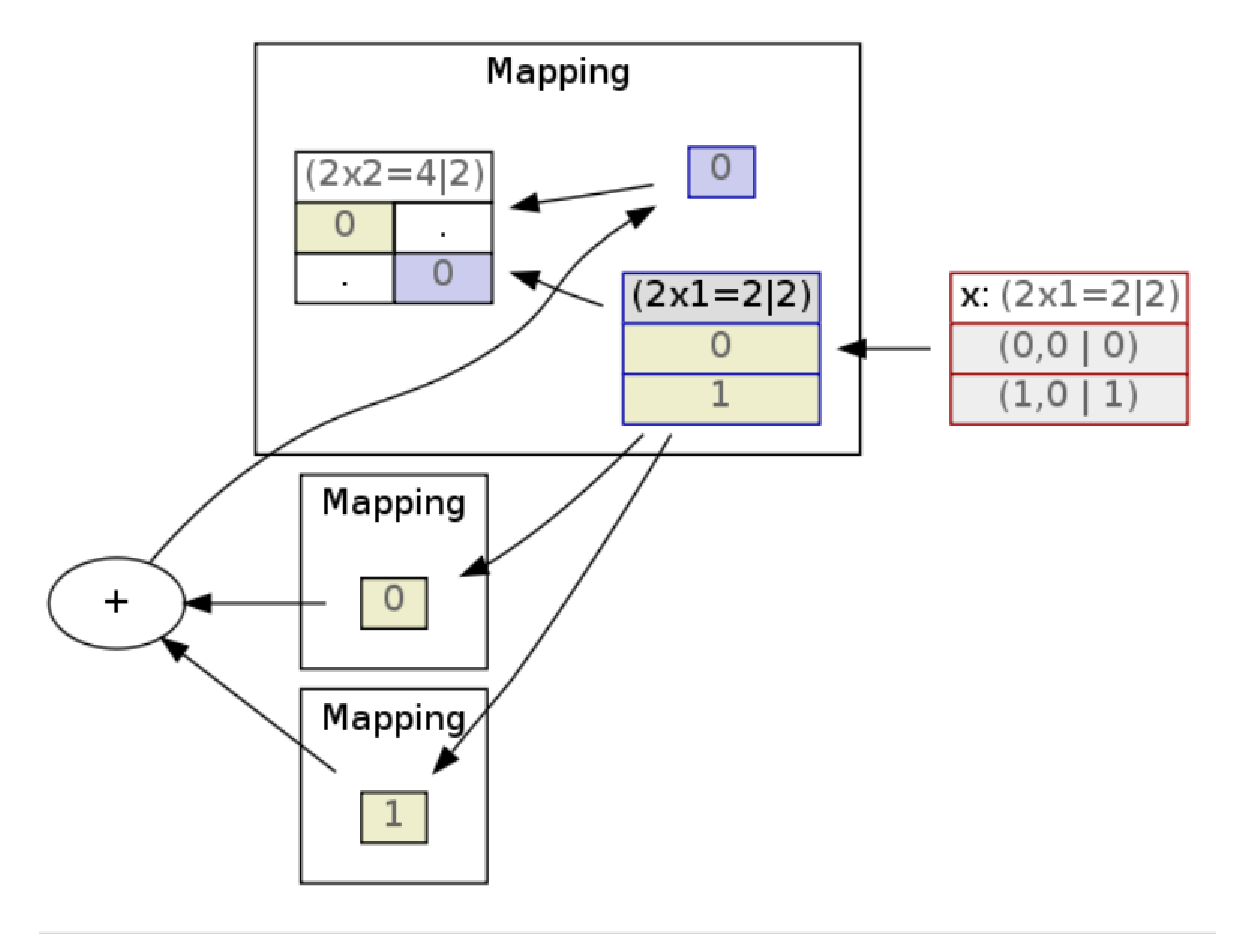
\includegraphics[width=0.8\textwidth]{mxdraw}
%% \end{center}

%% Using this feature, which is still under development, requires that you have installed the Python package \emph{pydot}. We actively work on getting the expressions easier to grasp.



%% \pytexStart{empty}

%% In \CasADi a powerful symbolic abstraction of mathematical functions is implemented.
%% In this chapter we will learn how to create general functions out of our model equations, 
%% how to evaluate them and optionally their derivatives. We also give some instructional
%% examples to make it more easily understandable.

%% The backbone of \CasADi is centered around some fundamental classes:
%% \begin{itemize}
%%  \item \texttt{SX} -- \emph{scalar symbolic type}
%%  \item \texttt{SX} -- \emph{sparse matrix with elements of type \texttt{SX}}
%%  \item \texttt{DMatrix}  -- \emph{same as \texttt{SX} but with elements of floating point type}
%%  \item \texttt{Function} and derived classes -- \emph{functions}
%%  \item \texttt{MX} -- \emph{matrix symbolic type}
%% \end{itemize}

%% \begin{pytexTemplate}{main}
%% from casadi import *
%% \end{pytexTemplate}

%% \begin{pytexTemplate}{maintools}
%% from casadi import *
%% from casadi.tools import *
%% \end{pytexTemplate}

%% \pytexStart{empty}

%% The following is a listing of available subclasses of Function:
%% \begin{pytex}
%% import casadi
%% import casadi.tools
%% casadi.tools.print_subclasses(casadi.Function)
%% \end{pytex}


\section{Mixing \texttt{SX} and \texttt{MX}}
You can \emph{not} multiply an \texttt{SX} object with an \texttt{MX} object, or perform any other operation to mix the two in the same expression graph. You can, however, in an \texttt{MX} graph include calls to a \emph{function} defined by \texttt{SX} expression. This will be demonstrated in Chapter~\ref{ch:function}. Mixing \texttt{SX} and \texttt{MX} is often a good idea since functions defined by \texttt{SX} expressions have a much lower overhead per operation making it much faster for operations that are naturally written as a sequence of scalar operations. The \texttt{SX} expressions is thus intended to be used for low level operations (for example the DAE right hand side, cf. Chapter~\ref{ch:integrators}), whereas the \texttt{MX} expressions act as a glue and enables the formulation of e.g. the constraint function of an NLP (which might contain calls to ODE/DAE integrators, or might simply be too large to expand as one big expression).

\section{The \texttt{Sparsity} class} \label{sec:sparsity_class}
As mentioned above, matrices in \CasADi are stored using the \emph{compressed column storage} (CCS) format. This is a standard format for sparse matrices that allows linear algebra operations such as elementwise operations, matrix multiplication and transposes to be performed efficiently. In the CCS, the sparsity pattern is decoded using the dimensions -- the number of rows and number of columns -- and two vectors. The first vector contains the index of the first structurally nonzero element of each column and the second vector contains the row index for every nonzero element. For more details on the CCS format, see e.g. \htmladdnormallink{Templates for the Solution of Linear Systems}{http://netlib.org/linalg/html_templates/node92.html} on Netlib. Note that \CasADi uses the CCS format for sparse as well as dense matrices.

Sparsity patterns in \CasADi are \emph{reference-counted}, meaning that multiple matrices can share the same sparsity pattern, including \texttt{MX} expression graphs and instances of \texttt{SX} and \texttt{DMatrix}. The \texttt{Sparsity} class is also \emph{cached}, meaning that the creation of multiple instances of the same sparsity patterns are (usually) avoided.

Like the matrix classes of \CasADi, the sparsity patterns are \emph{mutable} objects. This means e.g. that the patterns get updated when assigning a value to a structurally zero location of a matrix.

The following list summarizes the most commonly used ways of constructing new sparsity patterns:
\begin{description}
  \item[\texttt{Sparsity.dense}(\emph{n,m})]: Create a dense \emph{n}-by-\emph{m} sparsity pattern
  \item[\texttt{Sparsity.sparse}(\emph{n,m})]: Create a sparse \emph{n}-by-\emph{m} sparsity pattern
  \item[\texttt{Sparsity.diag}(\emph{n})]: Create a diagonal \emph{n}-by-\emph{n} sparsity pattern
  \item[\texttt{Sparsity.triu}(\emph{n})]: Create an upper triangular \emph{n}-by-\emph{n} sparsity pattern
  \item[\texttt{Sparsity.tril}(\emph{n})]: Create a lower triangular \emph{n}-by-\emph{n} sparsity pattern
\end{description}

The \texttt{Sparsity} class can be used to create non-standard matrices, e.g.
\begin{pytex}
print SX.sym("x",Sparsity.tril(3))
\end{pytex}

%% \chapter{Overview of operations}
%% In this chapter, we list the most central operations of \CasADi's symbolic framework. The list is not exhaustive, for more operations, search the API documentation or post a question in the \htmladdnormallink{forum}{http://forum.casadi.org/}.

%% \section{Creating sparsity patterns}
%% The following functions can be used to create new sparsity patterns:
%% \begin{description}
%%   \item[\texttt{Sparsity.dense}(\emph{nrow,ncol})]: Create a dense \emph{nrow}-by-\emph{ncol} pattern
%%   \item[\texttt{Sparsity.sparse(\emph{nrow,ncol})}]: Create a sparse \emph{nrow}-by-\emph{ncol} pattern
%%   \item[\texttt{Sparsity.diag(\emph{n})}]: Create a square \emph{n}-by-\emph{n} diagonal pattern
%%   \item[\texttt{Sparsity.triu(\emph{nrow,ncol})}]: Create a \emph{nrow}-by-\emph{ncol} upper triangular pattern
%% \end{description}

%% \section{Creating matrices}
%% The following functions can be used to create new matrices:
%% \begin{description}
%%   \item[\texttt{SX.sym}(\emph{name,n,m})]: Create a \emph{n}-by-\emph{m} symbolic primitive
%%   \item[\texttt{SX.zeros(\emph{n,m})}]: Create a \emph{n}-by-\emph{m} dense matrix with all zeros
%%   \item[\texttt{SX.sparse(\emph{n,m})}]: Create a \emph{n}-by-\emph{m} sparse matrix with all \emph{structural} zeros
%%   \item[\texttt{SX.ones(\emph{n,m})}]: Create a \emph{n}-by-\emph{m} dense matrix with all ones
%%   \item[\texttt{SX.repmat(\emph{v,n,m})}]: Repeat expression \emph{v} \emph{n} times vertically and \emph{m} times horizontally. \verb|SX.repmat(3,2,1)| will create a 2-by-1 matrix with all elements 3.
%%   \item[\texttt{SX.eye(\emph{n})}]: Create a \emph{n}-by-\emph{n} diagonal matrix with ones on the diagonal and structural zeros elsewhere.
%%   \item[\texttt{SX}(\emph{scalar})]: Create a scalar (1-by-1 matrix) with value \emph{scalar}. This method can be used explicitly, e.g. \verb|SX(9)|, or implicitly, e.g. \verb|9 * SX.ones(2,2)|.
%%   \item[\texttt{SX}(\emph{list})]: Create a column vector (n-by-1 matrix) with the elements in the list, e.g. \verb|SX([1,2,3])|
%%   \item[\texttt{SX}(\emph{list of lists})]: Create a dense matrix with the elements in the lists, e.g. \verb|SX([[1,2],[3,4]])|.
%% \end{description}

\section{Getting and setting elements in matrices} \label{sec:getset}
\CasADi offers a variety of different ways to get or set specific elements or blocks of elements in matrix types. There are two different categories for this:

\begin{description}
\item[Element access and assignment] Access or set elements of a matrix -- which may well be structural zeros --  by their (row, col) pairs. This is done with the syntax \verb|A = B[i,j]|, \verb|A[i,j] = B| in Python, and \verb|A = B(i,j)|, \verb|A(i,j) = B| in C++ and MATLAB.
\item[Nonzero access and assignment] Access or set a particular nonzero of the (sparse) matrices. Entries are ordered by columns using the compressed column storage format, cf. Section~\ref{sec:sparsity_class}. The syntax for this is \verb|A = B.el[k]|, \verb|A.el[k] = B| in Python, \verb|A = B[k]|, \verb|A[k] = B| in C++ and \verb|A = B{k}|, \verb|A{k} = B| in MATLAB.
\end{description}

In Python and C++, indexing starts from zero, while in MATLAB indexing starts from one. In Python, negative indices to specify an index counted from the end of a list.

The discussion in the following applies to all matrix types: \texttt{SX}, \texttt{MX}, \texttt{DMatrix}.

\subsection{Getting and setting}

%\pytexStart{main}

Each type of slicing comes with a get or set variant.
\begin{pytex}
M = DMatrix([[3,7],[4,5]])
print M[0,:]
\end{pytex}
\begin{pytex}
M[0,:] = 1
print M
\end{pytex}

Unlike NumPy, \CasADi slices are not views into the data of the left hand side; rather, a slice access copies the data. As a result, the matrix $M$ is not changed in the following example: 
%% \begin{pytex}
%% M = DMatrix([[3,7],[4,5]])
%% A = M[0,:]
%% A.set([1,1])
%% print A
%% print M
%% \end{pytex}

%% \begin{pytex}
%% M = DMatrix([[3,7],[4,5]])
%% M[0,:].set([1,1])
%% print M
%% \end{pytex}

\begin{pytex}
M = DMatrix([[3,7],[4,5]])
M[0,:][0,0] = 1 
print M
\end{pytex}

%\subsection{Flavors of slices}

\paragraph{Single element access} is getting or setting by providing a (\emph{row},\emph{column}) pair:
\begin{pytex}
M = diag([3,4,5,6])
print M
\end{pytex}
\begin{pytex}
print M[0,0]
\end{pytex}
\begin{pytex}
print M[1,0]
\end{pytex}
\begin{pytex}
print M[-1,-1]
\end{pytex}

Nonzero access works the same way:
\begin{pytex}
print M.nz[3]
\end{pytex}
\begin{pytex}
print M.nz[-2]
\end{pytex}

\paragraph{Slice access} means setting multiple elements at once. This is significantly more efficient than setting the elements one at a time. You get or set a slice by providing a (\emph{start},\emph{stop},\emph{step}) triple. In Python, \CasADi uses the standard syntax:
\begin{pytex}
print M[:,1]
\end{pytex}
which is equivalent to \verb|M(:,2)| in MATLAB and \verb|M(Slice(),1)| in C++.

\begin{pytex}
print M[1:,1:4:2]
\end{pytex}
which is equivalent to \verb|M(1:end,2:2:5)| in MATLAB and \verb|M(Slice(1,-1),Slice(1,4,2))| in C++.

\paragraph{List access} are similar to (but not as efficient as) slice access:
\begin{pytex}
M = DMatrix([[3,7,8,9],[4,5,6,1]])
print M
\end{pytex}
\begin{pytex}
print M[0,[0,3]]
\end{pytex}
\begin{pytex}
print M[[1,0],[0,3]]
\end{pytex}
\begin{pytex}
print M.nz[[6,1,3]]
\end{pytex}

%% \paragraph{Simple \emph{IMatrix} access} does repeated scalar access with a custom result shape. The user specifies \texttt{IMatrix}'es as item(s) in the rectangular brackets.  The result takes over the shape/sparsity of the supplied \texttt{IMatrix}.

%% In the \emph{nonzero access} style, each number of the \texttt{IMatrix} supplied is used as non-zero index into the left hand side matrix. In the \emph{full access} style, both \texttt{IMatrix}'es must have the same sparsity. Common non-zeros of the \texttt{IMatrix}'es form (row,col) pairs to access the left hand side.

%% \begin{pytex}
%% M = DMatrix([[3,7,8,9],[4,5,6,1]])
%% k = IMatrix([[0],[1]])
%% print M[k]    # [[3],[4]]
%% k = IMatrix([[0,1],[3,6]])
%% print M[k]    # [[3,  4 ],[5,  9 ]]
%% k = diag(range(4))
%% print M[k]    # diag([3,4,7,5])
%% \end{pytex}

%% \begin{pytex}
%% M = DMatrix([[3,7,8,9],[4,5,6,1]])
%% i = IMatrix([[0],[1]])
%% j = IMatrix([[2],[3]])
%% print M[i,j]    # [[8,1]]
%% i = diag([0,0,1,1])
%% j = diag([0,1,2,3])
%% print M[i,j]    # diag([3,7,6,1])
%% \end{pytex}

%% \paragraph{Mixed \texttt{IMatrix} access} deals with \emph{nonzero access} in a row or column wise fashion. Given a slice in the rows place and an \texttt{IMatrix} in the columns place, this flavor lets act \emph{simple \texttt{IMatrix} access} on each row individually. The results of all these \emph{simple \texttt{IMatrix} access} are concatenated vertically.

%% A similar definition holds for an IMatrix in the columns place, and a slice in the rows place of the double element rectangular bracket.

%% \begin{pytex}
%% M = DMatrix([[3,7,8,9],[4,5,6,1]])
%% j = IMatrix([[0],[1]])
%% print M[0,j]    # [[3],[7]]
%% print M[1,j]    # [[4],[5]]
%% print M[:,j]    # [[3],[7],[4],[5]]
%% \end{pytex}
%% \begin{pytex}
%% j = diag([0,2])
%% print M[:,j]    # [[3,  00 ],[00,  8 ],[4,  00 ],[00,  6 ]]
%% i = IMatrix([[0,1],[1,0]])
%% print M[i,:2]   # [[3,  4,  7,  5 ],[4,  3,  5,  7 ]]
%% \end{pytex}

%% \paragraph{Sparsity access} involves slicing with a sparsity pattern of the same shape as the left hand side. For each non-zero in the slice item, the element of the left hand side with the same (row, col) pair is selected.
%% \begin{pytex}
%% M = DMatrix([[3,7,8],[4,5,6],[1,2,9]])
%% print M[Sparsity.diag(3)]   # diag([3,5,9])
%% \end{pytex}


\section{Arithmetic operations}
\CasADi supports basic such as addition, multiplications, powers, trigonometric functions etc:
\begin{pytex}
x = SX.sym("x")
y = SX.sym("y",2,2)
print sin(y)-x
\end{pytex}

In C++ and Python, the standard multiplication operation (using \verb|*|) is reserved for elementwise multiplication. For \textbf{matrix multiplication}, use \verb|mul(A,B)|:
\begin{pytex}
print mul(y,y)
\end{pytex}

\textbf{Transposes} are formed using the syntax \verb|A.T| in Python or \verb|A.T()| in C++:
\begin{pytex}
print y.T
\end{pytex}

\textbf{Reshaping} means changing the number of rows and columns but retaining the number of elements and the relative location of the nonzeros. This is a cheap
 operation which is performed using the syntax:
\begin{pytex}
x = SX.eye(4)
print reshape(x,(2,8))
\end{pytex}

\textbf{Concatenation} means stacking matrices horizontally or vertically. Due to the column-major way of storing elements in \CasADi, it is efficient to stack matrices horizontally. Matrices that are in fact vectors (i.e. consisting of a single column), can also be stacked efficiently vertically. Vertical and horizontal concatenation is performed using the functions \texttt{vertcat} and \text{horzcat}, respectively:
\begin{pytex}
x = SX.sym("x",5,1)
y = SX.sym("y",5,1)
print vertcat((x,y))
\end{pytex}
\begin{pytex}
print horzcat((x,y))
\end{pytex}

\textbf{Horizontal and vertical splitting} are the inverse operations of the above introduced horizontal and vertical concatenation. To split up an expression horizontally into $n$ smaller expressions, you need to provide, in addition to the expression being splitted, a vector \emph{offset} of length $n+1$. The first element of the \emph{offset} vector must be 0 and the last element must be the number of columns. Remaining elements must follow in a non-decreasing order. The output $i$ of the splitting operation then contains the columns $c$ with $\textit{offset}[i] \le c < \textit{offset}[i+1]$. The following demonstrates the syntax:
\begin{pytex}
x = SX.sym("x",5,2)
offset = [0,1,2]
x1,x2 = horzsplit(x,offset)
print "x1 = ", x1, ", x2 = ", x2
\end{pytex}

The vertsplit operation works analogously, but with the \emph{offset} vector referring to rows:
\begin{pytex}
y = SX.sym("y",10,1)
offset = [0,5,10]
y1,y2 = vertsplit(y,offset)
print "y1 = ", y1, ", y2 = ", y2
\end{pytex}

It is always possible to use slice element access (cf. Section~\ref{sec:getset}) instead of horizontal and vertical splitting:
\begin{pytex}
y = SX.sym("y",10,1)
offset = [0,5,10]
y1,y2 = [y[offset[i]:offset[i+1],:] for i in range(len(offset)-1)]
print "y1 = ", y1, ", y2 = ", y2
\end{pytex}

For \texttt{SX} graphs, this alternative way is completely equivalent, but for \texttt{MX} graphs using \texttt{horzsplit}/\texttt{vertsplit} is \emph{significantly more efficient} and should be preferred when possible.

\textbf{Inner product}, defined as $<A,B> := \trace{A \, B} = \sum_{i,j} \, A_{i,j} \, B_{i,j}$ are created as follows:
\begin{pytex}
x = SX.sym("x",2,2)
print inner_prod(x,x)
\end{pytex}

Many of the above operations are also defined for the \texttt{Sparsity} class (Section~\ref{sec:sparsity_class}), e.g. \texttt{vertcat}, \texttt{horzsplit}, transposing, addition (which returns the \emph{union} of two sparsity patterns) and multiplication (which returns the \emph{intersection} of two sparsity patterns).

\section{Querying properties}
You can check if a matrix or sparsity pattern has a certain property by calling an appropriate member function. e.g. 
\begin{pytex}
y = SX.sym("y",10,1)
print y.shape
\end{pytex}

Some commonly used properties for a matrix \emph{A} are:
\begin{description}
  \item[\emph{A}.size1()] The number of rows
  \item[\emph{A}.size2()] The number of columns
  \item[\emph{A}.shape] The shape, i.e. the pair (\emph{nrow},\emph{ncol})
  \item[\emph{A}.numel()] The number of elements, i.e $\textit{nrow} * \textit{ncol}$
  \item[\emph{A}.size()] The number of structurally nonzero elements, equal to \emph{A}.numel() if \emph{dense}.
  \item[\emph{A}.sparsity()] Retrieve a reference to the sparsity pattern
  \item[\emph{A}.isDense()] Is a matrix dense, i.e. having no structural zeros
  \item[\emph{A}.isScalar()] Is the matrix a scalar, i.e. having dimensions 1-by-1?
  \item[\emph{A}.isVector()] Is the matrix a vector, i.e. having dimensions $n$-by-1?
  \item[\emph{A}.isSquare()] Is the matrix square?
  \item[\emph{A}.isTriu()] Is the matrix upper triangular?
  \item[\emph{A}.isConstant()] Are the matrix entries all constant?
  \item[\emph{A}.isInteger()] Are the matrix entries all integer-valued?
\end{description}

The last queries are examples of queries for which \emph{false negative} returns are allowed. A matrix for which \emph{A}.isConstant() is \emph{true} is guaranteed to be constant, but is \emph{not} guaranteed to be non-constant if \emph{A}.isConstant() is \emph{false}. We recommend you to check the API documentation for a particular function before using it for the first time.

\section{Linear algebra}
\CasADi supports a limited number of linear algebra operations, e.g. for solution of linear systems of equations:
\begin{pytex}
A = MX.sym("A",3,3)
b = MX.sym("b",3)
print solve(A,b)
\end{pytex}

\section{Calculus}
Basic calculus operations are also possibly and implemented very efficiently using \emph{algorithmic differentiation} (AD) as outlined in Chapter~\ref{ch:function}.
\begin{pytex}
A = SX.sym("A",3,3)
x = SX.sym("x",3)
print jacobian(mul(A,x),x)
\end{pytex}

%% \section{Sparsity tools}

%% Sparsities are easily visualized with the \texttt{spy} command:

%% \begin{pytex}
%% Sparsity.diag(3).spy()
%% \end{pytex}

%% \subsection{Sparsity constructors}
%% There are several options to build sparse \CasADi matrix types:

%% \begin{itemize}
%%  \item Start from an empty matrix and add elements by using indexing/slicing in a setting mode.
%%  \item Use sparsity constructors
%%  \item Convert from scipy sparse matrices
%% \end{itemize}

%% \begin{pytex}
%% print DMatrix.ones(Sparsity.tril(3))
%% print DMatrix(Sparsity.tril(3),range(6))
%% \end{pytex}

%% \paragraph{diagonal}
%% \begin{pytex}
%% Sparsity.diag(3).spy()
%% \end{pytex}

%% \paragraph{triangular}

%% \begin{pytex}
%% Sparsity.tril(3).spy()
%% \end{pytex}

%% \paragraph{banded}
%% \begin{pytex}
%% Sparsity.band(3,1).spy()
%% print ""
%% Sparsity.band(3,-1).spy()
%% \end{pytex}

%% \paragraph{row and column slices}
%% \begin{pytex}
%% Sparsity.rowcol([0,3],[1,2],4,4).spy()
%% \end{pytex}

%% \paragraph{(row,col) pairs}
%% \begin{pytex}
%% Sparsity.triplet(2,4,[0,1,0,0],[0,1,2,3]).spy()
%% \end{pytex}

%% \subsection{Sparsity operators}

%% The \texttt{+} operator is overloaded for sparsity patterns to perform an \emph{or} (pattern union) operation:
%% \begin{pytex}
%% (Sparsity.diag(3) + Sparsity.band(3,1)).spy()
%% \end{pytex}

%% The \texttt{*} operator is overloaded for sparsity patterns to perform an \emph{and} (pattern intersection) operation:
%% \begin{pytex}
%% (Sparsity.tril(4)*Sparsity.rowcol([2,3],range(4),4,4)).spy()
%% \end{pytex}



\chapter{Function objects} \label{ch:function}

\section{\texttt{Function} and derived classes} \label{sec:function}
\CasADi allows the user to create function objects, in C++ terminology often referred to as \emph{functors}, that all derive the \texttt{Function} base class. This includes functions that are defined by a symbolic expression, ODE/DAE integrators, QP solvers, NLP solvers etc.

The basic usage skeleton of all these function objects are\footnote{In C++, \texttt{getOutput} is return-by-reference}:
\begin{verbatim}
f = ClassName(arguments)                 # Call the constructor
f.setOption("option_name",option_value)  # Set options
f.init()                                 # Initialize the function
f.setInput(value,input_index)            # Pass inputs
f.evaluate()                             # Evaluate numerically
... = f.getOutput(output_index)          # Get outputs
\end{verbatim}

Note that all functions are multiple (sparse, matrix-valued) input, multiple (sparse, matrix-valued) output.

One important member of the \texttt{Function} derived classes is \texttt{SXFunction}, which is constructed with the syntax \texttt{SXFunction}(\emph{list of inputs},\emph{list of outputs}):
\begin{pytex}
x = SX.sym("x",2,2)
y = SX.sym("y")
f = SXFunction([x,y],[x,sin(y)*x])
\end{pytex}
which defines a function $f : \mathbb{R}^{2 \times 2} \times \mathbb{R}, \quad (x,y) \mapsto (x,\sin(y) x)$.

\texttt{MXFunction} works the same way, but for the \texttt{MX} expression graphs:
\begin{pytex}
x = MX.sym("x",2,2)
y = MX.sym("y")
f = MXFunction([x,y],[x,sin(y)*x])
\end{pytex}

%% We can get a list of other supported function objects deriving from \texttt{Function}:
%% \begin{pytex}
%% import casadi
%% import casadi.tools
%% casadi.tools.print_subclasses(casadi.Function)
%% \end{pytex}


%% There is no mechanism to distinguish the nature of \texttt{Function} functions. For example, any \texttt{Function} with \texttt{DAE\_NUM\_IN} inputs and \texttt{DAE\_NUM\_OUT} outputs can be considered to represent a dae function. The \CasADi used to generate this documentation has:
%% \begin{pytexoutput}
%% print "DAE_NUM_IN = ", DAE_NUM_IN
%% print "DAE_NUM_OUT = ", DAE_NUM_OUT
%% \end{pytexoutput}
%% There are a couple of global constants starting with \texttt{DAE\_} that together constitute the \emph{input/output scheme} of a dae. You can look these up in the API documentation or the python docstrings. You should use these constants and not replace them by the numerical values they happen to have in your version of \CasADi, as they might change in the future.\\

%% For example, here is an excerpt from the documentation for the constructor of a \texttt{CVodesIntegrator}:
%% \begin{pytexoutput}
%% docs = CVodesIntegrator.__init__.__doc__.split("\n")
%% start = docs.index(filter(lambda x: "DAEOutput" in x,docs)[0])
%% print "\n".join(docs[start:start+4+2*DAE_NUM_OUT])
%% \end{pytexoutput}

%% Helper functions are available to construct lists of objects that adhere to a particular scheme. For example, to create a list of a \texttt{DAEOutput} scheme, you use \texttt{daeOut}:

%% \begin{pytex}
%% print daeOut()
%% print daeOut(ode=SX.sym("function"))
%% print daeOut(alg=SX.sym("fz"),ode=SX.sym("function"))
%% \end{pytex}

%% Consult the python docstrings for more information of how to use these helper functions:
%% \begin{pytexoutput}
%% print daeOut.__doc__
%% \end{pytexoutput}

All derived classes of \texttt{Function} come with a range of options that can be set. The API documentation shows the list of available options for each class, along with their default values and descriptions.

%% For example, here is an excerpt from the documentation for \texttt{IpoptSolver}:
%% \begin{pytexoutput}
%% docs = IpoptSolver.__doc__.split("\n")
%% start = docs.index(filter(lambda x: "List of available monitors" in x,docs)[0])
%% print "\n".join(docs[start:start+15])
%% print "..."
%% \end{pytexoutput}

%% Two options commonly used during debugging, are "verbose" (a boolean) and "monitor". The latter allows to specify a list of keywords that each trigger some numerical output to be dumped to the screen when the function is evaluated. E.g. to monitor the objective and constraint function values during NLP solution, set:
%% \begin{verbatim}
%% solver.setOption("monitor",["eval_f","eval_g"])
%% \end{verbatim}

\section{Input-output schemes for function objects}
Most \texttt{Function}-derived classes have a particular input/output signature with them and/or take as arguments in the constructor other function objects (callback functions) with a particular input/output signature. For example, as we shall see in Chapter~\ref{ch:nlp}, a \emph{nonlinear program} (NLP) is defined by two inputs (the decision variable and a set of parameters) and two outputs (the objective and constraint functions). To make it easier to remember the number and order of the input/output arguments, \CasADi provides helper functions of the form:
\begin{pytex}
x = SX.sym("x")
p = SX.sym("p")
f = x*x
g = log(x)-p
nlp = SXFunction(nlpIn(x=x,p=p),nlpOut(f=f,g=g))
\end{pytex}

The last line is essentially equivalent to \verb|nlp = SXFunction([x,p],[f,g])|, but is preferred for a number of reasons:
\begin{itemize}
\item No need to remember the number or order of arguments
\item Inputs or outputs that are absent can be left unset
\item The helper functions provide meta-information that allows inputs to be referred to by their names instead of their index. E.g. \verb|nlp.jacobian("x","g")| instead of \verb|nlp.jacobian(0,1)|.
\end{itemize}

\section{Calling function objects}
\texttt{MX} expressions may contain calls to \texttt{Function}-derived functions. To embed a call to function (e.g. \texttt{SXFunction} or \texttt{Integrator}, see Chapter~\ref{ch:integrators}), you use the syntax:
\begin{verbatim}
[y1,y2,...,yn] = f([x1,x2,...,xn])
\end{verbatim}
That is, you provide a \emph{list} of argument expressions (which may consist of a single element) and gets back a list of expressions corresponding to the result of the call. Here is a code example:
\begin{pytex}
A = SX.sym("A",3,3)
x = SX.sym("x",3)
y = mul(A,x)
f = SXFunction([A,x],[y])
f.init()  # Must be called before symbolic or numeric evaluation

A2 = MX.sym("A",3,3)
x2 = MX.sym("x",3)
[y2] = f([A2,x2]) # Call f with argument (A2,x2)
\end{pytex}

Remember to put the brackets around the output even if the function only has a single output.

\section{Algorithmic differentiation}

The single most central functionality of \CasADi is \emph{algorithmic (or automatic) differentiation} (AD).

Assume a function $\mathbf{R}^N \rightarrow \mathbf{R}^M$:
\begin{equation}
 y = f(x)
\end{equation}

\emph{Forward mode} directional derivatives can be used to calculate Jacobian-times-vector products:
\begin{equation}
 y_{\text{fsens}} = \frac{\partial f}{\partial x} \, x_{\text{fseed}}
\end{equation}
We will refer to the multiplying vector as the \emph{seed} vector and the result as the \emph{sensitivity} vector.

Similarly, \emph{reverse mode} (or \emph{adjoint mode}) directional derivatives can be used to calculate Jacobian-transposed-times-vector products:
\begin{equation}
 x_{\text{asens}} = \left(\frac{\partial f}{\partial x}\right)^{\text{T}} \, y_{\text{aseed}}
\end{equation}

Both forward and adjoint directional derivatives are calculated at a cost proportional to evaluating $f(x)$, \emph{regardless of the dimension of $x$}.

CasADi is also able to generate complete, \emph{sparse} Jacobians efficiently. Internally, the algorithm it will use for this depends on the particular \texttt{Function} class but in most cases consists of the following steps:
\begin{itemize}
 \item Automatically detect the sparsity pattern of the Jacobian
 \item Use graph coloring techniques to find a few forward and/or directional derivatives needed to construct the complete Jacobian
 \item Calculate the directional derivatives numerically or symbolically
 \item Assemble the complete Jacobian
\end{itemize}

Hessians are calculated by first calculating the gradient and then performing the same steps as above to calculate the Jacobian of the gradient in the same way as above, while exploiting symmetry.

\section{Generating Jacobian and Hessian function objects}
You can generate a new function for calculating the Jacobian by calling the \texttt{Function::jacobian} member function:
\begin{verbatim}
 J = f.jacobian(iind,oind) # function corresponding to the jacobian
                           # of the oind-th output w.r.t. the iind-th input
\end{verbatim}
This will generate a function with the same input scheme as the function \texttt{f} but with the (sparse) Jacobian as well as all the original function outputs as outputs.

Similarly, the gradient of a scalar output can be called by calling the \texttt{Function::gradient} member function:
\begin{verbatim}
 G = f.gradient(iind,oind) # function corresponding to the gradient
                          # of the oind-th output w.r.t. the iind-th input
\end{verbatim}
which will generate a function with the same input scheme as the function \texttt{f} but with the (sparse) gradient and all the original function outputs as outputs.

Lastly, Hessians of a scalar output can be called by calling the \texttt{Function::hessian} member function:
\begin{verbatim}
 H = f.hessian(iind,oind) # function corresponding to the Hessian
                          # of the oind-th output w.r.t. the iind-th input
\end{verbatim}
which will generate a function with the same input scheme as the function \texttt{f} but with the (sparse) Hessian, the gradient and all the original function outputs as outputs.

\section{Converting \texttt{MXFunction} to \texttt{SXFunction}}
An \texttt{MXFunction} which only contains built-in operations (e.g. elementwise operations such as addition, square root, matrix multiplications and calls to \texttt{SXFunction} instances, can be converted into an \texttt{SXFunction} using the syntax:
\begin{verbatim}
 sx_function = SXFunction(mx_function)
\end{verbatim}

This might speed up the calculations significantly, but might also cause extra memory overhead.


%% \section{Calculating derivatives symbolically}
%% Directional derivatives can also be calculated symbolically, i.e. you can generate new expressions corresponding to directional derivatives for further manipulation. This is only possible for the \texttt{SXFunction} and \texttt{MXFunction} classes.
%% This is achieved by passing additional arguments to the \texttt{Function::eval} member function.

%% Similarly, expressions corresponding to complete Jacobians and Hessians can be obtained by calling the \texttt{SXFunction::jac} and \texttt{MXFunction::jac} functions.

%% We refer to the API documentation for details.

\chapter{ODE/DAE integration and sensitivity analysis} \label{ch:integrators}
\section{ODE/DAE formulation}
The integrators interfaced with \CasADi assumes a DAE residual function of semi-explicit form with quadratures:
\begin{subequations}
\begin{align}
 \dot{x} &= f_{\text{ode}}(t,x,z,p), \qquad x(0) = x_0 \\
      0  &= f_{\text{alg}}(t,x,z,p) \\
 \dot{q} &= f_{\text{quad}}(t,x,z,p), \qquad q(0) = 0
\end{align}
\end{subequations}

For solvers of \emph{ordinary} differential equations, the second equation and the algebraic variables $z$ must be absent.

%% \newcommand{\backward}[1]{#1^*}
%% \begin{equation}
%%   \begin{array}{l}
%%     f:
%%     \mathbb{R}^{n_x} \times \mathbb{R}^{n_u}
%%     \times \mathbb{R}^{n_r} \times \mathbb{R}^{n_v}
%%     \rightarrow  
%%     \mathbb{R}^{n_x} \times \mathbb{R}^{n_q}
%%     \times \mathbb{R}^{n_r} \times \mathbb{R}^{n_p}, \\
%%     \quad (x_0, u, r_1, v) \mapsto (x_1, q_1, r_0, p_0) \\
%%     \noalign{\smallskip}
%%     \left\{
%%     \begin{array}{rcl}
%%      \dot{x}(t) &=& \phi(x(t),z(t),u), \\
%%               0 &=& \theta(x(t),z(t),u), \\
%%      \dot{q}(t) &=& \psi(x(t),z(t),u), \\
%%     -\dot{r}(t) &=& \backward{\phi}(x(t),z(t),u,r(t),s(t),v), \\
%%               0 &=& \backward{\theta}(x(t),z(t),u,r(t),s(t),v), \\
%%     -\dot{p}(t) &=& \backward{\psi}(x(t),z(t),u,r(t),s(t),v),
%%     \end{array}
%%     \right. 
%%      ~~~~~~~~~~~~~~~~~~~~~~~~~~~~~t \in [0,1], \\
%%      \noalign{\smallskip}
%%      x(0) = x_0, \quad r(1) = r_1, \quad q(0) = 0, \quad p(1) = 0, \\
%%      \noalign{\smallskip}
%%      x_1 = x(1), \quad q_1 = q(1), \quad r_0 = r(0), \quad p_0 = p(0),
%%   \end{array}
%% \end{equation}

DAEs of form can be formed using the \verb|daeIn| and \verb|daeOut| helper functions:

\begin{pytex}
x = SX.sym("x")
z = SX.sym("z")
f = -z*x
g = z*z-2
dae = SXFunction(daeIn(x=x,z=z),daeOut(ode=f,alg=g))
print dae
\end{pytex}

%This particular problem is actually troublesome. During integration, the rootfinding problem $C(z) = 0$ will be solved, and the initial guess is $z=0$. Since $\frac{dC}{dz}(z=0)=0$, the rootfinding will fail. You cannot force a different initial guess directly, but you can transform the $z$ variable:
%$z \rightarrow z + 1$ -- $C=z^2+2z-1$, which will work fine.

An integrator in \CasADi is a function that take the state at the initial time, a set of parameters, the state vector at the initial time and a guess for the algebraic variables (only for DAEs) and returns the state vector and algebraic variables at the final time. 
\begin{verbatim}
integrator = Integrator("solver_name",dae)
\end{verbatim}

The time horizon is assumed to be fixed\footnote{for problems with free end time, you can always scale time by introducing an extra parameter and substitute $t$ for a dimensionless time variable that goes from 0 to 1} and can be set with the option:
\begin{verbatim}
 integrator.setOption("tf",integration_end_time)
\end{verbatim}

\section{Sundials integrators}
The Sundials suite contains the two popular integrators CVodes and IDAS for ODEs and DAEs respectively. These two integrators supports forward and adjoint sensitivities and when used via \CasADi's Sundials interface, \CasADi will automatically formulate the Jacobian information, which is needed by the backward differentiation formula (BDF) that CVodes and IDAS use. Also automatically formulated will be the forward and adjoint sensitivity equations. This means that the only information that the user needs to provide is the DAE residual function:
\begin{verbatim}
 integrator = Integrator("cvodes",dae)  # For ODEs
 integrator = Integrator("idas",dae)    # For DAEs
\end{verbatim}
for CVodes and IDAS respectively.

For a list of options for the integrators, as well as the input and output schemes of this \emph{function}, check the documentation directly from Python:
\begin{verbatim}
print Integrator.doc("cvodes")
\end{verbatim}
or by consulting the online C++ API docs on the website.

\section{Sensitivity analysis}
From evaluation point of view, an integrator behaves just like the \texttt{SXFunction} introduced in the previous session. You set inputs, forward/adjoint seeds, evaluate and obtain the outputs and forward/adjoint sensitivities.

\section{The \texttt{Simulator} class}
As already mentioned, integrators in \CasADi are functions that calculates the state at the final time. Often, however, a user is interested in obtaining the solution at multiple time points. This can often be done more efficiently than by repeatedly calling \texttt{integrator.evaluate()}. The easiest way to use this functionality is to use the \texttt{Simulator} class.

A \texttt{Simulator} can be created using the syntax:
\begin{verbatim}
  # Import numpy
  import numpy as NP

  # Allocate an integrator instance
  integrator = ...
  integrator.setOption("...",...)

  # Choose a time grid
  tgrid = NP.linspace(0,end_time,num_time_steps)

  # Create a simulator
  simulator = Simulator(integrator, time_grid)
\end{verbatim}

A \texttt{Simulator} can be used just like an integrator, and its input scheme is the same. Its output is now matrix valued, with the the columns corresponding to different time points. The class can also be used to evaluate a particular function of the state at a set of time points. See the API documentation for more information.

\chapter{Nonlinear Programming} \label{ch:nlp}
The NLP solvers contained in or interfaced with \CasADi solves parametric NLPs of the following form:
\begin{equation}
\begin{array}{cc}
\begin{array}{c}
\text{minimize:} \\
x \in \mathbb{R}^{nx}, p \in \mathbb{R}^{np}
\end{array}
&
f(x,p)
\\
\begin{array}{c}
\text{subject to:}
\end{array}
&
\begin{array}{c}
x_{\min} \le x \le x_{\max} \\
g_{\min} \le g(x,p) \le g_{\max}
\end{array}
\end{array}
\end{equation}

With a function \texttt{nlp}, which given $x$ and $p$, gives $f$ and $g$, an NLP solver instance can be allocated by:
\begin{verbatim}
 nlp_solver = NlpSolver("solver_name",nlp)
\end{verbatim}

The interface will then automatically generate the information that it might need to solve the NLP, which may be solver and option dependent. Typically an NLP solver will need a function that gives the Jacobian of the constraint function and a Hessian of the Lagrangian function ($L(x,\lambda) = f(x) + \lambda^{\text{T}} \, g(x))$ with respect to $x$. The interface will generate this kind of information automatically and provide to the solver.

NLP solvers, like ODE/DAE integrators are functions in \CasADi (though taking derivatives of them is currently not supported). You will find the input and output schemes in the \CasADi API documentation on the website or by using the question mark in Python.

\chapter{Optimal control with \CasADi}
\CasADi can be used to solve \emph{optimal control problems} (OCP) using a variety of methods, including direct (a.k.a. \emph{discretize-then-optimize}) and indirect (a.k.a. \emph{optimize-then-discretize}) methods, all-at-once (e.g. collocation) methods and shooting-methods requiring embedded solvers of initial value problems in ODE or DAE. As a user, you are in general expected to \emph{write your own OCP solver} and \CasADi aims as making this as easy as possible by providing powerful high-level building blocks. Since you are writing the solver yourself (rather than calling an existing ``black-box'' solver), a basic understanding of how to solve OCPs is indispensable. Good, self-contained introductions to numerical optimal control can be found in the recent textbooks by Biegler\footnote{Lorenz T. Biegler, \emph{\htmladdnormallink{Nonlinear Programming: Concepts, Algorithms, and Applications to Chemical Processes}{http://books.google.es/books/about/Nonlinear_Programming.html?id=VdB1wJQu0sgC&redir_esc=y}}, SIAM 2010} or Betts\footnote{John T. Betts, \emph{\htmladdnormallink{Practical Methods for Optimal Control Using Nonlinear Programming}{http://books.google.es/books/about/Practical_Methods_for_Optimal_Control_Us.html?id=Yn53JcYAeaoC&redir_esc=y}}, SIAM 2001} or Moritz Diehl's lecture notes on \htmladdnormallink{numerical optimal control}{http://homes.esat.kuleuven.be/~mdiehl/NUMOPT/numopt.pdf}.

\section{Optimization of a Van der Pol oscillator}
In \CasADi's examples collection\footnote{You can obtain this collection as an archive named \texttt{examples\_pack.zip} in \CasADi's \htmladdnormallink{download area}{http://files.casadi.org}}, you find codes for solving simple optimal control problem using a variety of different methods. The problem is driving a \emph{Van der Pol} oscillator to the origin, while trying to minimize a quadratic cost:
\begin{equation}
\begin{array}{lc}
\begin{array}{l}
\text{minimize:} \\
x(\cdot) \in \mathbb{R}^2, \, u(\cdot) \in \mathbb{R}
\end{array}
\quad \displaystyle \int_{t=0}^{10}{(x_0^2 + x_1^2 + u^2) \, dt}
\\
\\
\text{subject to:} \\
\\
\begin{array}{ll}
\left\{
\begin{array}{l}
\dot{x}_0 = (1-x_1^2) \, x_0 - x_1 + u \\
\dot{x}_1 = x_0 \\
-0.75 \le u \le 1.0
\end{array} \right. & \text{for $0 \le t \le 10$} \\
x_0(0)=0, \quad x_0(10)=0  \\
x_1(0)=1, \quad x_1(10)=0  
\end{array}
\end{array}
\label{eq:vdp}
\end{equation}

\section{Direct single-shooting}
The simplest OCP method to implement in \CasADi is single-shooting. In fact, it can be implemented in just 30 lines of code, which the script {\texttt{vdp\_single\_shooting.py}} in \CasADi's examples collection demonstrates. Please go through the code carefully and make sure that you understand the principle. The most important part of the code are the lines:
\begin{verbatim}
# Build a graph of integrator calls
for k in range(nk):
  X, = integratorOut(integrator(integratorIn(x0=X,p=U[k])),"xf")
\end{verbatim}

Here, we recursively construct a symbolic expression for the state at the final time. This expression is then used in the formulation of the NLP objective and constraint functions.

\section{Direct multiple-shooting}
The second optimal control method we shall consider is multiple shooting. In multiple shooting, the states at each ''shooting node'' are degrees of freedom in the NLP. The script \\ \texttt{vdp\_multiple\_shooting.py} demonstrates how the VDP problem can be solved using direct multiple shooting in \CasADi.

Note how the symbolic variable in the NLP functions now contains both the control and states for each of the \texttt{nk} intervals:
\begin{verbatim}
# Total number of variables
nv = 1*nk + 3*(nk+1)

# Declare variable vector
V = MX.sym("V", nv)
\end{verbatim}

Also note how the recursive overwriting of \texttt{X} has been replaced with:
\begin{verbatim}
for k in range(nk):
  # Local state vector
  Xk = vertcat((X0[k],X1[k],X2[k]))
  Xk_next = vertcat((X0[k+1],X1[k+1],X2[k+1]))
  
  # Call the integrator
  Xk_end, = integratorOut(integrator(integratorIn(x0=Xk,p=U[k])),"xf")
  
  # append continuity constraints
  g.append(Xk_next - Xk_end)
  g_min.append(NP.zeros(Xk.size()))
  g_max.append(NP.zeros(Xk.size()))
\end{verbatim}

\section{Direct collocation}
When we went from direct single shooting to direct multiple shooting we essentially traded nonlinearity for problem size. The NLP in single shooting is small, but often highly nonlinear, whereas the NLP for multiple-shooting is larger, but less nonlinear and with a sparsity structure that can be exploited efficiently. Direct collocation is to take one more step in the same direction, adding even more degrees of freedom. The resulting NLP is even larger, but has even more structure that can be exploited.

While multiple shooting only includes the state at the beginning of each control interval as a degree of freedom in the NLP (in addition to the discretized control and the parameters), in direct collocation the state at a set of \emph{collocation points} (in addition to the beginning of the interval) enters in the NLP as variables. An example of a choice of time points are the \emph{Legendre points} of order $d=3$ :
\begin{equation}
 \tau = [0,0.112702,0.500000,0.887298]
\end{equation}

Keeping the same control discretization as in single and multiple shooting:
\begin{equation}
 u(t) = u_k, \quad \text{for $t \in [t_k, t_{k+1}], \quad k=0,\ldots,n_k-1$}
\end{equation}

the complete list of time points, with $h_k := t_{k+1}-t_k$, is:
\begin{equation}
 t_{k,j} := t_k + h_k \, \tau_j, \quad \text{for $k=0,\ldots,n_k-1$ and $j=0,\ldots,d$}
\end{equation}
as well as the final time $t_{n_k,0}$. Also let $x_{k,j}$ denote the states at these time points.

On each control interval, we shall define a Lagrangian polynomial basis:
\begin{equation}
 L_j(\tau) = \prod_{r=0, \, r \ne j}^{d} \frac{\tau - \tau_{r}}{\tau_j - \tau_r}
\end{equation}

Since the Lagrangian basis satisfies:
\begin{equation}
 L_j(\tau_r) = \left\{
 \begin{array}{l}
  1, \qquad \text{if $j=r$} \\
  0, \qquad \text{otherwise}
 \end{array}
  \right.
\end{equation}
we can approximate the state trajectory approximation as a linear combination of these basis functions:
\begin{equation}
\tilde{x}_k(t) = \sum_{r=0}^{d}{L_r\left(\frac{t-t_k}{h_k}\right) \, x_{k,r}}
\end{equation}

In particular we get approximations of the state time derivative at each collocation point (not including $\tau_0$):
\begin{equation}
\tilde{\dot{x}}_k(t_{k,j}) = \frac{1}{h_k} \, \sum_{r=0}^{d}{\dot{L}_r(\tau_j) \, x_{k,r}} := \frac{1}{h_k} \, \sum_{r=0}^{d}{C_{r,j} \, x_{k,r}}
\label{eq:colldef}
\end{equation}

as well as an approximation of the state at the end of the control interval:
\begin{equation}
\tilde{x}_{k+1,0} = \sum_{r=0}^{d}{L_r(1) \, x_{k,r}} := \sum_{r=0}^{d}{D_r \, x_{k,r}}
\label{eq:contdef}
\end{equation}

Plugging in the approximation of the state derivative (\ref{eq:colldef}) into the ODE gives us a set of \emph{collocation equations} that needs to be satisfied for every state at every collocation point:
\begin{equation}
h_k \, f(t_{k,j},x_{k,j},u_k) - \sum_{r=0}^{d}{C_{r,j} \, x_{k,r}} = 0, \qquad k=0,\ldots,n_k-1, \quad j=1,\ldots,d
\end{equation}

And the approximation of the end state (\ref{eq:contdef}) gives us a set of \emph{continuity equations} that must be satisfied for every control interval:
\begin{equation}
x_{k+1,0} - \sum_{r=0}^{d}{D_r \, x_{k,r}} = 0, \qquad k=0,\ldots,n_k-1, 
\end{equation}

These two sets of equations take the place of the continuity equation (represented by the integrator call) in direct multiple shooting. The above equations have been implemented in the script \texttt{vdp\_collocation.py}.

\chapter{Import and reformulation of OCPs from Modelica} \label{ch:modelica}
\CasADi supports importing OCPs formulated in the Modelica modeling language as well as in the Optimica extension of Modelica to optimal control. The import facility currently works with the open-source \htmladdnormallink{JModelica.org}{http://www.jmodelica.org/} compiler.

For instructions on how to install and use JModelica.org, we refer to their \htmladdnormallink{website}{http://www.jmodelica.org/}. Note that a \CasADi build (which may not be the latest) is contained in the pre-built JModelica.org binaries.

\emph{NOTE: The functionality to import and reformulation of OCPs from Modelica is still under development and to be considered unstable.}

\section{Compiling the Modelica code} \label{sec:modelica_compilation}
To see how to use the Modelica import, look at \htmladdnormallink{thermodynamics\_example.py}{https://github.com/casadi/casadi/blob/tested/examples/python/modelica/fritzson_application_examples/thermodynamics_example.py} and \htmladdnormallink{cstr.cpp}{https://github.com/casadi/casadi/blob/tested/examples/cplusplus/cstr.cpp} in \CasADi's example collection. 

Assuming that the Modelica/Optimica model \texttt{ModelicaClass.ModelicaModel} is defined in the files \texttt{file1.mo} and \texttt{file2.mop}, the compile command is:
\begin{verbatim}
  from pymodelica import compile_jmu
  jmu_name=compile_jmu('ModelicaClass.ModelicaModel', \
    ['file1.mo','file2.mop'],'auto','ipopt',\
    {'generate_xml_equations':True, 'generate_fmi_me_xml':False})
\end{verbatim}

This will generate a \texttt{jmu}-file, which is essentially a zip file containing, among other things, the file \texttt{modelDescription.xml}. This XML-file contains a symbolic representation of the optimal control problem and can be inspected in a standard XML editor.
\begin{verbatim}
  from zipfile import ZipFile
  sfile = ZipFile(jmu_name','r')
  mfile = sfile.extract('modelDescription.xml','.')
\end{verbatim}

\section{The SymbolicOCP class} \label{sec:modelica_import}
The symbolic optimal control problem representation (or just model description) contained in \texttt{modelDescription.xml} can be imported into \CasADi in the form of the SymbolicOCP class:
\begin{verbatim}
ocp = SymbolicOCP()
\end{verbatim}

The \texttt{SymbolicOCP} class contains symbolic representation of the optimal control problem designed to be general and allow manipulation. The basic usage of this class is to call the member function \texttt{parseFMI} with the XML file name:
\begin{verbatim}
ocp.parseFMI('modelDescription.xml')
\end{verbatim}

Symbolic expressions corresponding to the states, controls parameters etc. are directly accessible as member variables of the \texttt{SymbolicOCP} object. E.g. the free controls can be accessed as \verb|ocp.u|. Symbolic expressions for the OCP are either accessible in the same way (e.g. \verb|ocp.dae| will return the equations for the fully-implicit differential-algebraic equation formulation used by Modelica. Other equations are tied to a particular variable. E.g. the \emph{binding equations} corresponding to the set of \emph{independent parameters} can be retrieved as \verb|ocp.beq(ocp.pi)|. 

Other useful commands available for an instance \texttt{ocp} of \texttt{SymbolicOCP} include:
\begin{description}
\item[print \texttt{ocp}] Print the optimal optimal control problem to screen
\item[\texttt{ocp}.makeExplicit()] Reformulate the OCP in fully-explicit form
\item[\texttt{ocp}.scaleVariable()] Scale all variables using the \emph{nominal} attribute for each variable
\item[\texttt{ocp}.eliminateIndependentParameters()] Eliminate all independent parameters from the symbolic expressions
\end{description}

For a more detailed description of this class and its functionalities, we refer to the API documentation. We also recommend potential users to have a look at the {\texttt{modelica\_ms.py}} tutorial example.

\chapter{Syntax differences between \CasADi in Python, C++ and MATLAB (in development)} \label{ch:syntax_differences}
\scriptsize
\begin{center}
  \begin{tabular}{| p{3.5cm} | p{3.5cm} | p{3.5cm} | p{3.5cm} | }
    \hline
      & Python & C++ & MATLAB (in development) \\ \hline
    Starting \CasADi & \verb|from casadi import *| & \verb|#include \| \verb|"casadi/casadi.hpp"| \verb|using namespace casadi;| & \verb|import casadi.*| \\ \hline
    Printing the \emph{representation} (string representation intended to be \emph{unambiguous}) & \verb|A <ENTER>| (interactive), \verb|print repr(A)| (in scripts) & \verb|std::cout << A;|& \verb|A <ENTER>| or \verb|disp A|\\ \hline
    Printing the \emph{description} (string representation intended to be \emph{readable}) & \verb|print A| & \verb|A.print();| or \verb|A.print(stream);|& \verb|A.print()| \\ \hline
    Calling a class function & \verb|SX.zeros(3,4)| & \verb|SX::zeros(3,4)| & \verb|SX.zeros(3,4)|\\ \hline
    Element access & \verb|A[i,j]|, \emph{0-based} & \verb|A(i,j)| and \verb|A(i)|, \emph{0-based} & \verb|A(i,j)|, \emph{1-based} \\ \hline
    Element assignment & \verb|A[i,j] = b|, \emph{0-based} & \verb|A(i,j) = b| and \verb|A(i) = b|, \linebreak \emph{0-based} & \verb|A(i,j) = b|, \emph{1-based} \\ \hline
    Nonzero access & \verb|A.el[k]|, \emph{0-based} & \verb|A[k]|, \emph{0-based} & \verb|A{k}|, \emph{1-based} \\ \hline
    Nonzero assignment & \verb|A.el[k] = b|, \emph{0-based} & \verb|A[k] = b|, \emph{0-based} & \verb|A{k} = b|, \emph{1-based} \\ \hline
    Matrix multiplication & \verb|mul(x,y)| & \verb|mul(x,y)| & \verb|mul(x,y)| or \verb|x*y| \\ \hline
    Elementwise multiplication & \verb|x*y| & \verb|x*y| & \verb|x.*y| \\ \hline
    Elementwise division & \verb|x/y| & \verb|x/y| & \verb|x./y| \\ \hline
    Power & \verb|x**y| & \verb|pow(x,y)| & \verb|x^y| or \verb|x.^y| \\ \hline
    Transpose & \verb|transpose(A)| or \verb|A.T| & \verb|transpose(A)| or \verb|A.T()|& \verb|transpose(A)| or \verb|A'| or \verb|A.'| \\ \hline
    Creating a dictionary (e.g. for options) & \verb|d = {'opt1':opt1}| or \verb|d = {}; a['opt1'] = opt1| & \verb|a = Dictionary();| \verb|a['opt1'] = opt1;| & \verb|a = Dictionary();| \verb|a('opt1') = opt1;| \\ \hline
    Getting function output by value & \verb|out = f.getOutput()| & \verb|DMatrix out;| \verb|f.getOutput(out);| & \verb|out = f.getOutput()| \\ \hline
  \end{tabular}
\end{center}

%\bibliographystyle{plain}
%\bibliography{ug_cites}
\end{document}
